\chapter{Discusión}\label{discusion}

\section{Metodología de trabajo}

En todo proyecto no solo es importante el resultado, sino el camino que lleva a éste último. Durante el desarrollo del proyecto se utilizó la metodología ágil SCRUM, la cual consta a grandes rasgos de una pila Backlog de requerimientos, Sprints correspondientes a intervalos acotados de trabajos destinados a cumplir una cierta porción de los requerimientos y reuniones bastante más consecutivas que con otras metodologías. 

Para las especificaciones del proyecto se hizo bastante cómodo su uso, pues grandes cambios suponían solo modificar ciertos Sprint y en caso de encontrar problemas o bloqueantes, por la comunicación frecuente dentro del equipo se podían tomar decisiones en un corto periodo de tiempo.

\begin{figure}[H]
	\centering
	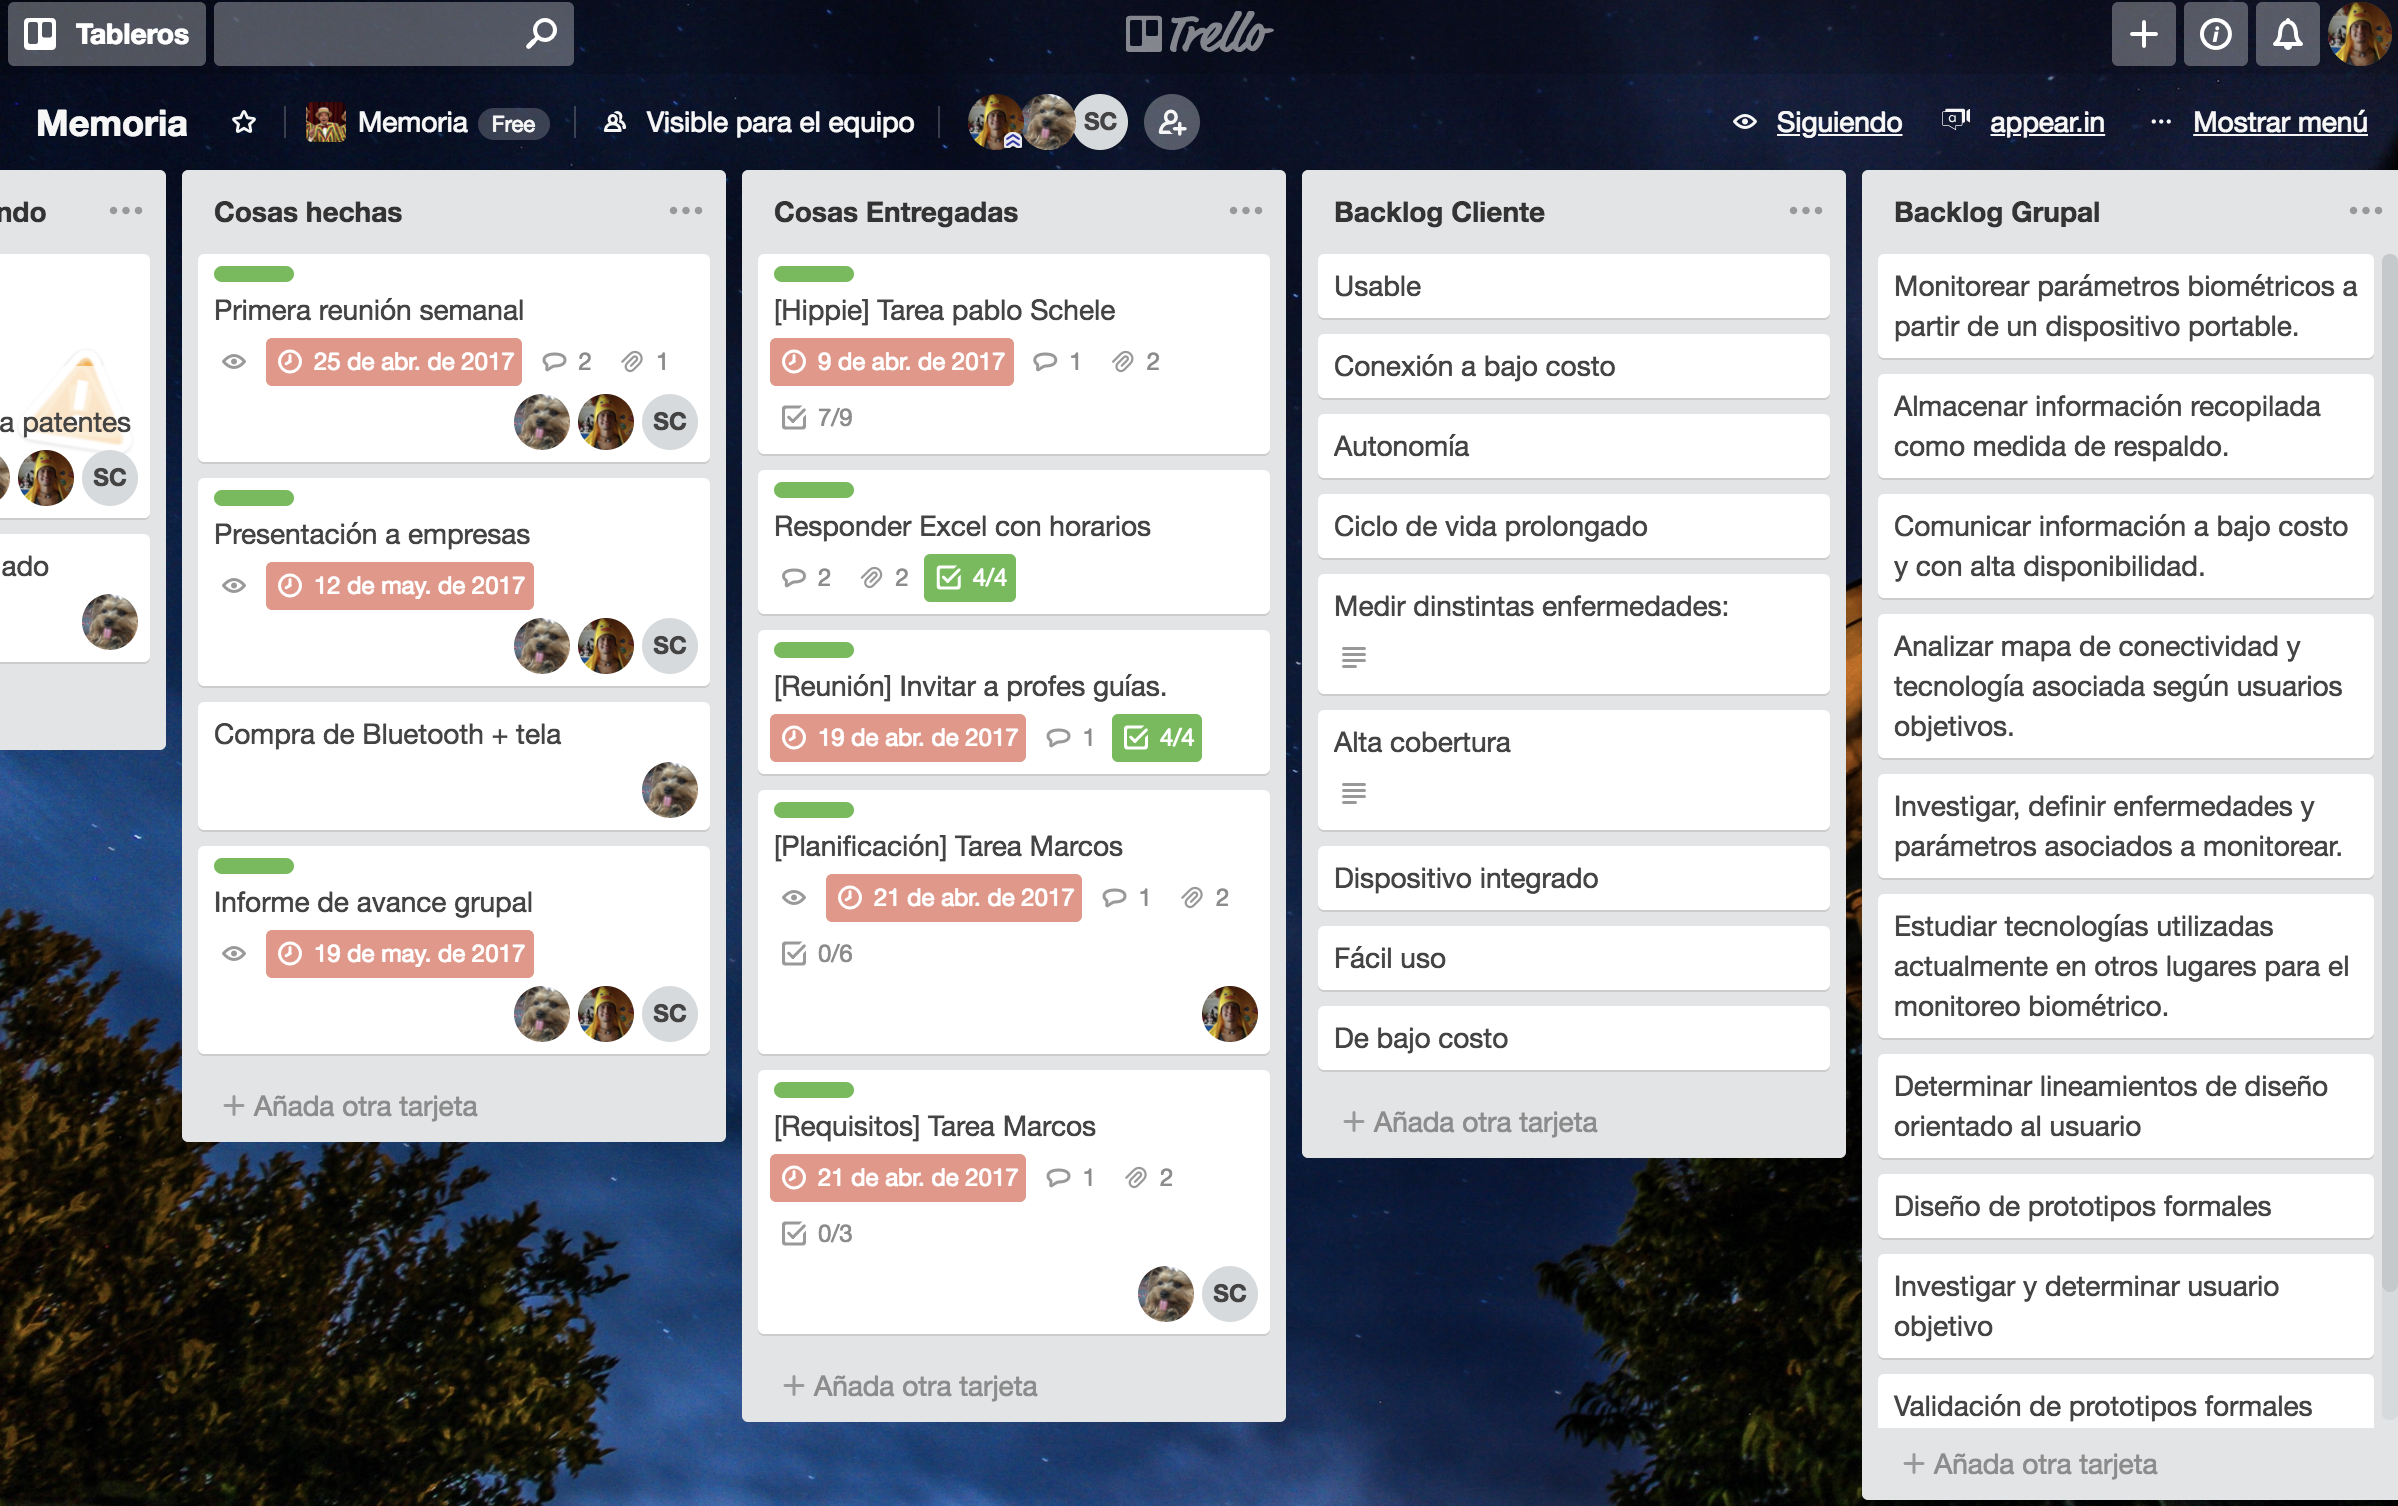
\includegraphics[scale=0.28]{figuras/discusion/trello.png}
	\caption{Tableros empleados en Trello}
	\label{trello}
\end{figure}


Para llevar a cabo la organización se hizo uso de Trello, una plataforma de organización laboral común, en tiempo real y basada en la nube, la cual permite el seguimiento de los distintos avances y trabajos de cada uno de los integrantes del equipo. Como se puede observar en la figura \ref{trello} es posible trabajar en base a tableros, listas y tarjetas (uno contenedor de otro respectivamente).


\section{Relaciones públicas}

Durante el transcurso del proyecto se hizo patente la necesidad de contactar con actores reales que enfrentaran problemáticas asociadas. Por este motivo, se realizaron contactos con distintos profesionales en búsqueda de información y/o alianzas:

\textbf{Proyecto Almohadita}: Proyecto de monitoreo y clasificación de riesgo intrahospitalario a distancia. Implementado en el hospital Dr. Exequiel González Cortés y a cargo de Sebastián Ríos, Investigador ISCI (Instituto de Sistemas Complejos de Ingeniería) Académico FCFM (Facultad de Ciencias Físicas y Matemáticas) U Chile. 

No se logró establecer una reunión formal con el equipo desarrollador de este proyecto, su relevancia yacía en la cercanía con los objetivos entre los proyectos (monitoreo a distancia).

\textbf{SubTel}: En un unicio se estableció contacto con la Subsecretaría de Telecomunicaciones con el fin de obtener información de cobertura nacional de las distintas bandas celulares disponibles. 

Dando como resultado la ley de Neutralidad de la red, respuesta adjunta en los anexos.

\newpage

\textbf{Profesionales de la Salud}: Se contactó con la enfermera jefa de urgencias Elizabeth Nievas, y los doctores Fabián Álvarez (Jefe de Urgencias) y Cristian Mondaca (Jefe del programa salud cardiovascular y jefe de farmacia). Todos del hospital de Quintero Adriana Cousiño, con los cuales se contrastaron requerimientos y se barajó la factibilidad de realizar pruebas con pacientes.

La información recopilada permitió un lineamiento más cercano del proyecto a la realidad (cantidad de derivaciones necesarias, entre otros).

\textbf{DesafIoT (3IE)}: Durante el verano de 2018, se fue partícipe como equipo multidisciplinario del desafío propuesto por la incubadora de la Universidad Federico Santa María 3IE. El cual estaba destinado a equipos con desarrollos de proyectos con tecnología IoT (Internet of Things). 

No fue posible continuar con el programa, principalmente por aspectos económicos del proyecto (poca viabilidad por falta de clientes actuales e interesados) y del poco interés generado hacia los jueces de la propuesta (falta de innovación).

\section{Trabajos futuros}

Con lo presentado en los anteriores capítulos se logró obtener un MVP (Minimum viable product) en respuesta a lo pedido por la contraparte, las expectativas del equipo y lo esperado por el programa de memorias multidisciplinarias. Sin embargo, es importante al menos nombrar ciertos aspectos que como equipo consideramos importantes o a tener en cuenta como trabajos futuros:

\textbf{Frecuencia cardiaca}: A partir del ECG es posible recuperar la frecuencia cardiaca aislando los pick de la señal.

\textbf{Sincronización de Base de datos}: Generar la lógica capaz de sincronizar las bases de datos (a partir de la comunicación ya configurada).

\textbf{Patrón de diseño}: Como proyecto de desarrollo en Android, es posible mejorar su mantenimiento con un patrón de diseño como MVP\cite{mvp} o MVVM\cite{mvvm} (para programación reactiva).

\textbf{Mejoras visuales}: Una mejora en el diseño visual de la aplicación móvil permitiría una mayor aceptación por parte de los usuarios y posibles inversores (como con Material Design).

\textbf{Documentación de código}: A partir de generadores de documentación como Doxygen, es posible dar un soporte más completo al código fuente.

\textbf{Buenas prácticas}: Algunas como empleo de StringBuffer o StringBuilder en reemplazo de una concatenación directa de cadenas de texto, referenciar a null al terminar de utilizar un objeto, para que el recolector de Java libere los recursos, entre otros.

\textbf{Análisis de resultados}: Análisis de parámetros como ancho de banda, tiempo de respuesta o tamaño de almacenamiento en Base de datos, son resultados calculables y que no se lograron abarcar por el tiempo de desarrollo.

\textbf{Optimizar código Arduino}: En desmedro del tiempo de respuesta asociado al microcontrolador se podría aumentar la tasa de transferencias significativamente, pues se le daría prioridad a los envíos por sobre el análisis de las peticiones Bluetooth.

\textbf{Encriptación de Base de datos}: Debido a la sensibilidad de los datos, es relevante verificar la factibilidad de encriptar los datos almacenados, tanto locales como remotos. Aunque siempre cuidando el impacto en el desempeño final.

\textbf{ProGuard}\cite{proguard}: En algún punto del desarrollo podría darse el caso de tener en el código fuente información sensible, por lo que un método de ocultación como lo es la ofuscación a través de ProGuard para Android es un método simple y efectivo (aunque el tiempo de compilación aumenta considerablemente, por lo que su uso solo sería para versiones de producción).

\newpage

\section{Nuevas tecnologías y su impacto en el proyecto}

En el mundo de la programación y específicamente la programación móvil, siempre existen cambios menores y grandes cada cierto tiempo. Por lo que con tan solo un año podría generarse un cambio rotundo que afectara a un proyecto completo, como lo pueden ser nuevas herramientas, nuevos lenguajes, nuevas librerías o esquemas visuales.

En este sentido, se hace una recopilación de tecnologías relevantes para un proyecto de esta índole y se analiza su impacto de ser implementadas. Debido a la naturaleza del proyecto desarrollado, esta recopilación se centrará en Android principalmente aunque no de forma exclusiva.

\textbf{Actualización Java}\cite{java8}: En Abril de 2015 se hizo patente la versión de Java 8, con cambios tan significativos como nuevas funciones de las interfaces o expresiones lambda. Cambios que son capaces de ser portados a Android desde su versión 7.0 (API 24) en adelante. El uso de expresiones lambda permitiría disminuir ciertas funciones menores no reutilizables.

\textbf{Mensajes binarios}: Con miras en el rendimiento en la comunicación, el uso de mensajes binarios en contraste con mensajes de cadenas de texto permitiría una mejora importante en las tasas de transferencia (aunque habría que verificar la compatibilidad con las herramientas empleadas).

\textbf{Flutter}\cite{flutter}: La nueva propuesta de Google en el desarrollo híbrido no ha dejado indiferente a nadie y es posible que sea uno de los grandes cambios en el desarrollo móvil de los últimos años. En el proyecto esto permitiría la generación de versiones móviles tanto para iOS como para Android, a partir de un mismo código fuente y posiblemente en un menor tiempo que el desarrolado de forma nativa, pues se define a sí mismo como: ``UI Framework para la creación de experiencias nativas en Android y iOS en tiempo récord".

\newpage

\textbf{Kotlin}\cite{kotlin}: El nuevo lenguaje diseñado por JetBrains propone una actualización al lenguaje Java al poder correr sobre la máquina virtual de este lenguaje y es oficialmente utilizado en el desarrollo Android. Entre sus ventajas se encuentra la disminución de código generado y por ende un mantenimiento más amigable, además de soporte para programación funcional.

\textbf{HTTP/2 + SSE (Server-Sent Events)}\cite{http2sse}: La combinación del nuevo protocolo HTTP/2 y SSE permite una comunicación bidireccional como con Websocket, aunque obligando al uso de encriptación y con la característica de compresión de cabeceras, además de una multiplexación en la comunicación (agilizando las respuestas). No se considera un reemplazo, por lo que su impacto no sería tan directo como cabe esperar pero es una tendencia que cabe tener en cuenta.

\textbf{Pruebas Unitarias}\cite{unittest}: El desarrollo de una aplicación móvil se puede realizar de distintas maneras, bajo distintos patrones y a gusto del programador, pero si se quiere realizar pruebas unitarias (al menos en Android), se requiere desde un principio tener la perspectiva para programar módulos capaces de responder de forma independiente. Como ganancia, se tiene una aplicación altamente escalable, modularizada y de fácil mantenimiento/actualización.

\textbf{Integración continua}: La integración continua es una práctica de desarrollo software donde los miembros del equipo integran su trabajo frecuentemente (como mínimo una vez al día, aunque normalmente se realizan múltiples integraciones diarias).
Cada integración se verifica compilando el código fuente y obteniendo un ejecutable (a esto se le llama build, y debe hacerse de forma automatizada).Además también se pasan las pruebas y métricas de calidad para detectar los errores tan pronto como sea posible. El programa por excelencia en este aspecto es Jenkins\cite{jenkins}.

\newpage

\textbf{Inspección continua}: Como su nombre indica, informa continuamente sobre código duplicado, estándares de codificación, pruebas unitarias, cobertura de código, complejidad ciclomática, potenciales errores, comentarios y diseño del software. En el breve periodo de desarrollo no es posible imaginar su uso de forma frecuente, pero sí es importante destacarlo como herramienta para proyectos de mayor envergadura (y por consiguiente con mayor tiempo de desarrollo) y su mayor exponente es SonarQube\cite{sonarqube}.

\textbf{Machine Learning}: En los últimos años se ha hecho patente el uso de técnicas de Machine Learning para multitud de problemas, dentro de los cuales destaca la medicina por ser un campo común a la sociedad. En este sentido, el poder de predicción y análisis de datos que ofrecen herramientas como TensorFlow\cite{tensor}, MxNet\cite{mxnet} o Matlab dotarían de potencia al proyecto. Permitiendo incluso, convertirlo en un proyecto con capacidades de detección/aviso propias, sin tener que ser necesariamente consultado por un médico. 

\textbf{BlockChain}: Junto con las criptomonedas, el uso de esta tecnología ha escalado en los últimos años y detrás de su faceta financiera se esconden características impresionantes. La capacidad de tener una base de datos distribuida, descentralizada, encriptada y de difícil manipulación malintencionada (dependerá de la cantidad de nodos presentes en la red) la hacen una gran candidata para ser la base de datos del futuro, ofreciendo confianza y velocidad (al no tener que verificar por terceros las distintas operaciones realizadas en la base de datos) a los usuarios.
